\documentclass[12pt]{article}

% page setup
\usepackage[a5paper, landscape, bottom=1cm]{geometry}
\pagenumbering{gobble}

% encoding & language
\usepackage{selinput}
\SelectInputMappings{}
\usepackage[T1]{fontenc}
\usepackage[ngerman]{babel}
\usepackage[babel, german=quotes]{csquotes}

% text
\usepackage{parskip}
\usepackage[lighttt]{lmodern}
\usepackage{setspace}
\onehalfspacing

% images
\usepackage{graphicx}

\begin{document}

\section*{Aufgabe 1}

\begin{enumerate}
    \item Modellieren Sie folgendes Diagramm:
\end{enumerate}

\begin{figure}[hbt]
    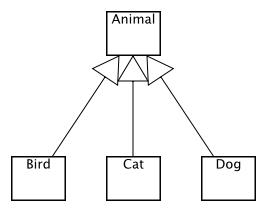
\includegraphics[scale=1]{assets/exercise-1}
\end{figure}

\newpage

\section*{Aufgabe 2}

\begin{enumerate}
    \item Erstellen Sie eine Klasse \texttt{\textbf{Bicycle}}.
    \item Fügen Sie der Klasse \texttt{\textbf{Bicycle}} eine neue Oberklasse \texttt{\textbf{Vehicle}} hinzu.
    \item Erstellen Sie eine neue Klasse \texttt{\textbf{Driver}}.
    \item Fügen Sie der Klasse \texttt{\textbf{Vehicle}} eine neue Unterklasse \texttt{\textbf{Car}} hinzu.
    \item Fügen Sie der Klasse \texttt{\textbf{Vehicle}} eine neue Unterklasse \texttt{\textbf{Train}} hinzu.
    \item Nennen Sie die Klasse \texttt{\textbf{Bicycle}} zu \texttt{\textbf{Bike}} um.
    \item Fügen Sie der Klasse \texttt{\textbf{Car}} eine neue Unterklasse \texttt{\textbf{Van}} hinzu.
\end{enumerate}

\newpage

\section*{Aufgabe 3A}

\begin{enumerate}
    \item Modellieren Sie folgendes Diagramm:
\end{enumerate}

\begin{figure}[h]
    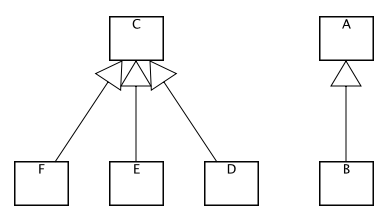
\includegraphics[scale=0.9]{assets/exercise-3a}
\end{figure}

\newpage

\section*{Aufgabe 3B}

\begin{enumerate}
    \setcounter{enumi}{1}
    \item Verändern Sie nun das modellierte Diagramm, so dass es wie folgt aussieht:
\end{enumerate}

\begin{figure}[h]
    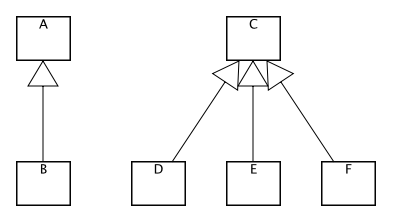
\includegraphics[scale=0.9]{assets/exercise-3b}
\end{figure}

\newpage

\section*{Aufgabe 4}

In dieser Aufgabe soll eine Vererbungshierarchie für geometrische Objekte erstellt werden. Die Oberklasse der Hierarchie soll \texttt{\textbf{Shape}} genannt werden. Die Objekte werden in zwei- und dreidimensionale Objekte aufgeteilt, die durch die Klassen \texttt{\textbf{Shape2D}} und \texttt{\textbf{Shape3D}} repräsentiert werden. Beide Klassen sind Unterklassen der Klasse \texttt{\textbf{Shape}}.

Zu den zweidimensionalen Objekten gehören Ellipse (Klasse \texttt{\textbf{Ellipse}}) und Polygon (Klasse \texttt{\textbf{Polygon}}). Eine spezielle Form der Ellipse, der Kreis, soll durch die Klasse \texttt{\textbf{Circle}} repräsentiert werden. Zu den Polygonen gehören Rechteck (Klasse \texttt{\textbf{Rectangle}}) und Dreieck (Klasse \texttt{\textbf{Triangle}}). Eine spezielle Form des Rechtecks, das Quadrat, soll durch die Klasse \texttt{\textbf{Square}} repräsentiert werden.

Zu den dreidimensionalen Objekten gehören Kugel (Klasse \texttt{\textbf{Sphere}}), Pyramide (Klasse \texttt{\textbf{Pyramid}}), Quader (Klasse \texttt{\textbf{Cuboid}}), Zylinder (Klasse \texttt{\textbf{Cylinder}}) und Kegel (Klasse \texttt{\textbf{Cone}}). Eine spezielle Form des Quaders, der Würfel, soll mit der Klasse \texttt{\textbf{Cube}} repräsentiert werden.

Sortieren Sie anschließend die erstellten Klassen im Diagramm alphabetisch.

\end{document}
